\documentclass{article}
\usepackage{graphicx} % Required for inserting images
\usepackage[utf8]{inputenc}
\usepackage{color}
\newcommand{\hello}{Hello Latex. This is from new command}
\newcommand{\greetings}[3]{Hello #1. This is #2 and I am #3.}

\usepackage[T1]{fontenc}
%https://www.overleaf.com/learn/latex/font_typefaces
\usepackage{tgbonum}
\usepackage{amsmath}

\begin{document}

%\frontmatter	 
\title {\bf{ASSIGNMENT} }
\date{\today}
%\maketitle

  %\begin{titlepage}
  %\section{ASSIGNEMENT}

    \let\footnotesize\small
    \let\footnoterule\relax
    \let \footnote \thanks
    \setcounter{footnote}{0}
    
    %\begin{center}
    \maketitle

  %\begin{titlepage}
  %\section{ASSIGNEMENT}

    \let\footnotesize\small
    \let\footnoterule\relax
    \let \footnote \thanks
    \setcounter{footnote}{0}
    
    \begin{center}

     
       
\includegraphics[width=2.8cm]{aust-logo.png}

{\Large \bf Ahsanullah University of Science and 
Technology\linebreak}
      \smallskip
      { \Large \bf \ Course Title :- Introduction to Computer system Lab \par}
      {\Large \bf Course no: CSE1108  \linebreak}
      \smallskip
      
     {\Large \bf Topic: ``Artificial Intelligence'' \linebreak}
     {\Large \bf Date of submission:- 22/02/2022 \linebreak}
     

      %{\large in \par}
      
       {\Large \em Submitted by \par}
      \smallskip
      {\LARGE \bf Ahnaf Amer\linebreak}
      {\large \bf ID:- 20220104040 \linebreak}
      \linebreak
      {\LARGE \bf Atik Shahrier Ullash \linebreak}
      {\large \bf ID:- 20220104034 \linebreak}
	{\large \bf 1$^{st}$ Year,1$^{st}$ Semester \par}
 {\large \bf LAB Group;-A2 \par}
 
 {\Large \em Submitted to \par}
{\LARGE \bf Tammana Tabbasum \linebreak}
{\large \bf Lecturer\par}
{\large \bf Department of CSE,AUST\par}


        \end{center}
\newpage



\newpage
 %\begin{c}
     
 %\end{center}
 

 
   {\Large \bf \underbar{Contents}  }
  % \begin{document}
\section{ Introduction to Artificial Intelligence
}


\section{History of Artificial intelligence}
\section{Uses of Artificial Intelligence
}
\section{Disadvantages of Artificial Intelligence}

.\par
%\end{center}

\newpage

%\titleformat{
% {\normalfont\Large\sffamily\bfseries\filcenter}%{\uline{\Introduction to Artificial Intelligence\hspace*{ 1em}}}{0em}%{\uline{\MakeUppercase{#1}}}}

\renewcommand*{\thesection}{\Roman{section}}
%\marketitle
%\{ Introduction to Artificial Intelligence
%}

\noindent\LARGE\bf{\underbar{1.Introduction to Artificial Intelligence}}\par\smallskip


\noindent 
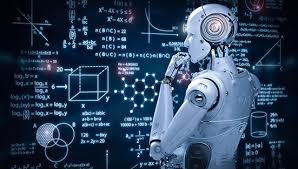
\includegraphics[width=12cm]{Artificial intelligence.jpg}\par
 {\large \bf AI (Artificial Intelligence) is a machine’s ability to perform cognitive functions as humans do, such as perceiving, learning, reasoning, and solving problems. The benchmark for AI is the human level concerning in teams of reasoning, speech, and vision. Artificial Intelligence is the type of intelligence which is not found naturally but created through high level of programming and research.\par

The word ‘Artificial’ in AI can awaken much different associations. It can bring forth the fear of cyborgs. It reminds us of the images from science fiction novels.Well, that fear might not be too far from the truth. Well, Artificial Intelligence is a type of Intelligence which is comparable to the intelligence of Human (Artificial Intelligence have not reached the intelligence level of human but it might only be a few decades before they reach this spot. For example: Robot Sophia) which means these intelligence makes the owner of the intelligence to think for themselves and take the decision for themselves. So, if they are not treated well, our worst nightmare might come true. Anyway, the main point is Artificial Intelligence is a type of intelligence created artificially which is comparable to the intelligence of humans.
   \par \linebreak}
  
 
 
%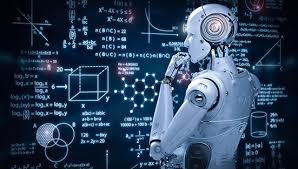
\includegraphics[width=10cm]{Artificial intelligence.jpg}\par
\newpage

%\subsection{History of artificial intelligence}
\noindent \textbf{\underbar{2.History of Artificial Intelligence }}
\linebreak\
\noindent 
{\large \bf The history of artificial intelligence (AI) began in antiquity, with myths, stories and rumors of artificial beings endowed with intelligence or consciousness by master craftsmen.\par 

The most recent history of Artificial Intelligence can be invention of the programmable digital computer in the 1940s, a machine based on the abstract essence of mathematical reasoning. This invention and its way of work encouraged the scientists to try and make an electronic brain which will be able to think for itself and take decision without the need of outside help. The field of AI research was founded in 1956 at a workshop held on the campus of Dartmouth College, USA. The scientist who attended this workshop become the leader of AI research in the future. They also predicted that in the near future, a machine capable of intelligence like humans will exist and they were given a lot of money to make this vision come true. But the scientists and investors underestimated the difficulty of this project and soon in the 1970s the funding for research of Artificial Intelligence was withdrawn by the US and British Governments. As a result, work on developing artificial intelligence was mostly stopped and interest about AI lowered a lot until the 21st century. An effort was done by the Japanese Government in the meantime using a huge amount of money but which also failed due to the difficulty of the project. In the 21st century investment and interest bloomed in Ai when machine learning was successfully applied to many problems in academia and industry due to new methods, the application of powerful computer hardware, and the collection of immense data sets.\par 

It is true that the development of artificial intelligence is mainly done in the modern history. But it doesn’t mean the concept of artificial intelligence is a modern thing. The concept of AI can be found in many ancient mythologies like the Greek mythology.
  

 %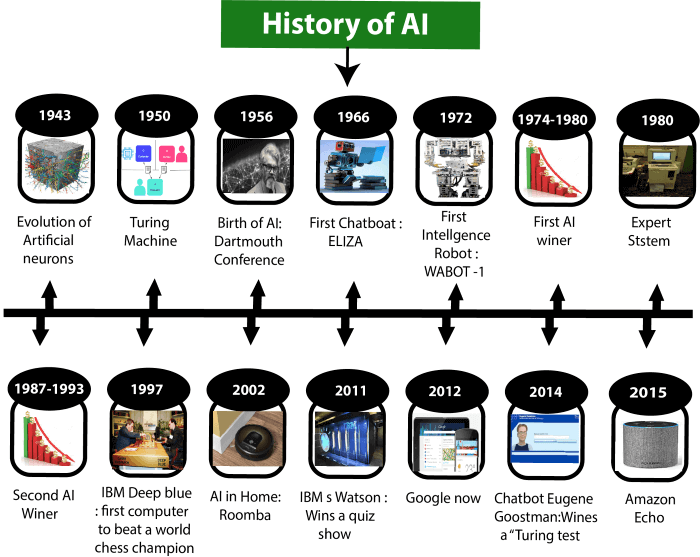
\includegraphics[width=8cm]{History of AI.png}\par
 %\caption{Figure-1:History of A.I}
 %\linebreak
 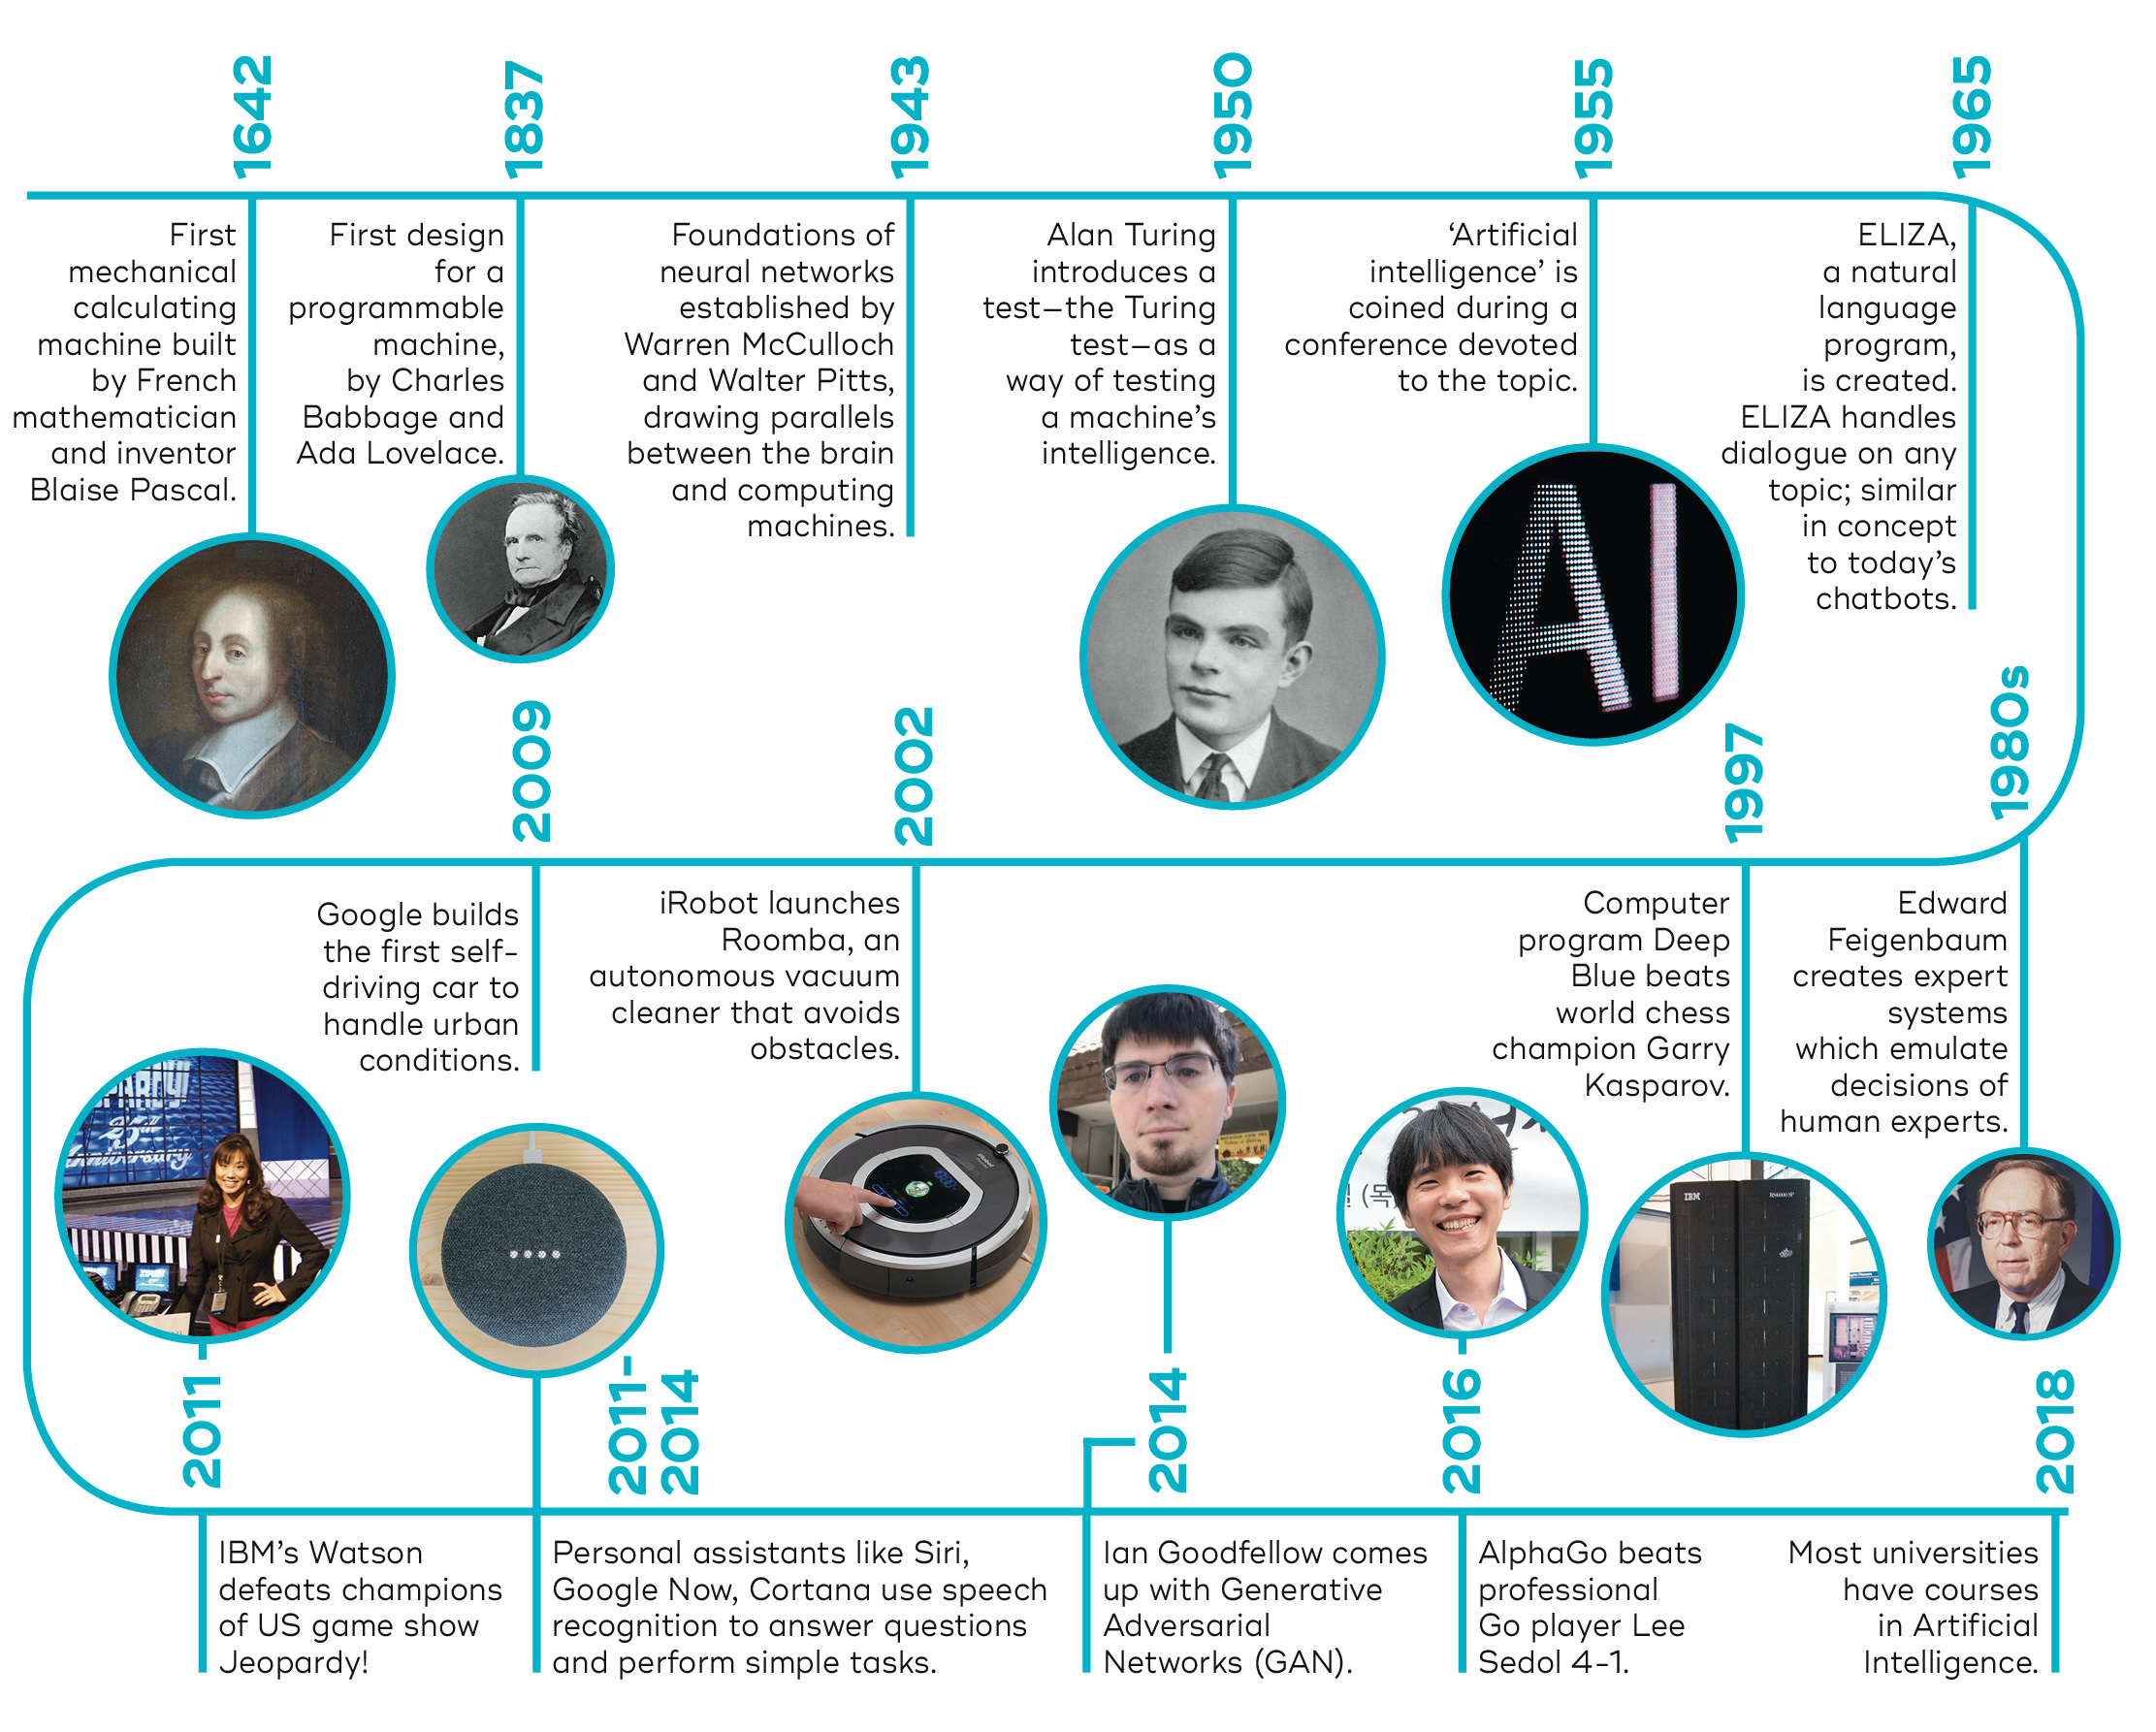
\includegraphics[width=12cm]{History Of AI 2.jpg}\par
 \centering
  \caption{Figure:History of A.I }\smallskip
\par\linebreak}


\linebreak 
%\smallskip
\noindent

\noindent \textbf{\underbar{3.Uses of Artificial Intelligence}}

\noindent \textbf{Artificial Intelligence is now a big part of life. It is used in every part of life. A few uses of artificial intelligence is given below:}

\begin{enumerate}
\item  \textbf{\underbar{Medicine:} Artificial intelligence are used extensively in medical sciences. Common uses are diagnosing patients, drug discovery and development, communication between doctor and patients, prescribing medicines for well-known diseases etc.\underbar{}}

\item \textbf{\underbar{ Education:} One of the big uses of Artificial intelligence are in the field of education. Creating study material, sharing them, delivering information to all people even tutoring is some of its uses.\underbar{}}

\item \textbf{\underbar{ Communication:} Artificial Intelligence is used for communication also. Artificial intelligence is not used actively but it is still for various purposes like selecting route for travelling, booking ticket, learning of the weather etc.\underbar{}}

\item \textbf{\underbar{ Business:} AI is used for many reason in Business. Some of this reasons are} \textbf{spam filters, smart email categorization, voice to text features, smart personal assistants, such as Siri, Cortana and Google Now, automated responders and online customer support, process automation etc.}

\item \textbf{ \underbar{Daily life uses:} We use artificial almost at all times of our daily lives. They have made our daily life far easier than ever before. Some of those uses are Personalized Shopping, AI-Powered Assistants, fraud Prevention, Administrative tasks Automated to Aid educators, creating smart content, voice Assistants, personalized learning etc.}
\end{enumerate}
\centering
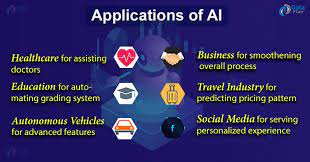
\includegraphics[width=12cm]{uses of AI.jpg}\par

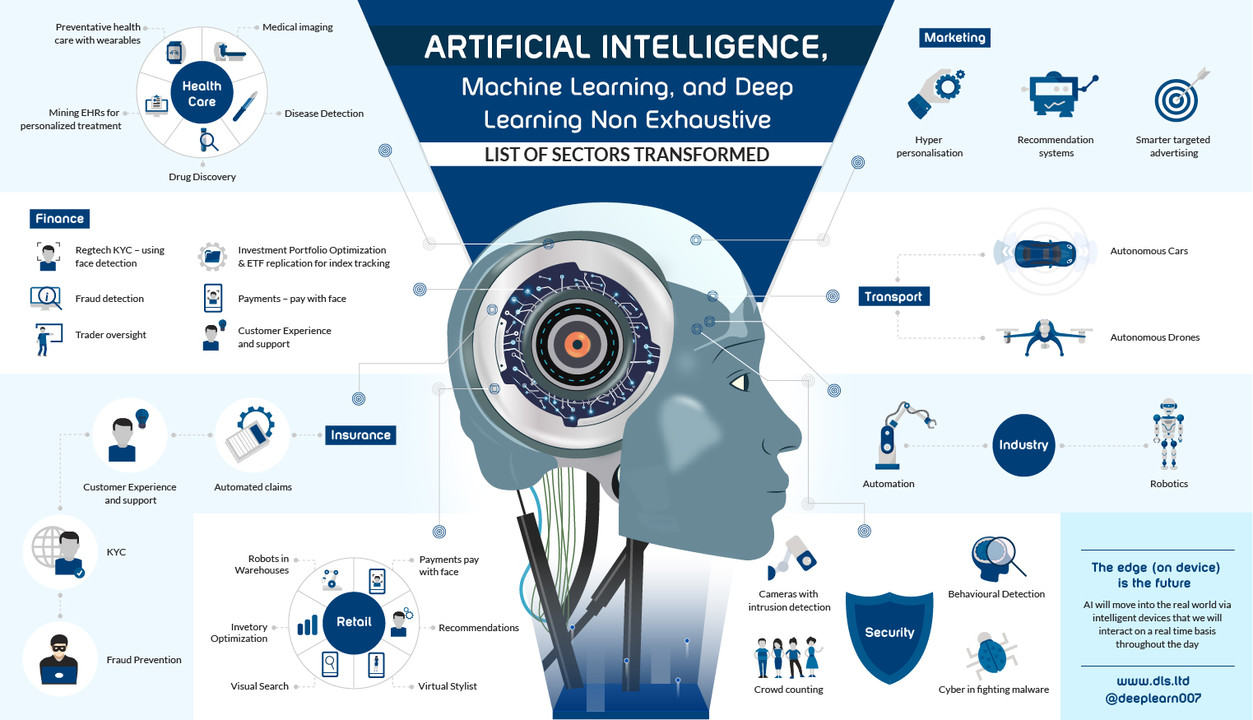
\includegraphics[width=12cm]{uses of AI 2.jpg}\par
\centering
 \bf\large\caption{Figures of uses of AI}
 % \par\linebreak}
 
\noindent

\newpage
\noindent \textbf{\underbar{4. Disadvantages of Artificial Intelligence:~}}

\noindent \textbf{As there are many uses of Artificial Intelligence, it has many disadvantages as well which cannot be overlooked. Some of them are as follows:}

\begin{enumerate}
\item  \textbf{\underbar{High production cost:~ }Artificial intelligence is an artificial thing as said before as it is created by humans. It helps a lot in our lives, but it takes a lot of money and time to develop it which is very valuable in our age. So, it makes you think `Is it really worth it to create AI?'\underbar{}}

\item \textbf{\underbar{ Responsible for unemployment issue: }AI is the intelligence of a machine capable of thinking. Now-a-days, AI is used in all sorts of machines. As a result, the performance of the machines increased as they could do the same work as people and for long amount of time. As a result, AI took over for a lot of jobs. But, in doing so, it escalated a problem we are trying to solve for a long time, Unemployment problem. Because of AI, now unemployment problem has reached sky-high and we are not able to find any suitable solution to it.\underbar{}}

\item \textbf{\underbar{ Emotionless machines: }AI is currently at a state where it has started to form mentality like people but those are only a few. Most of the AI's still work just as they are programmed. And as difficult complex programming is not used, these AI's are unable to have emotion, which makes nothing more or less that a puppet.\underbar{}}
\end{enumerate}

\noindent 

%\noindent \textbf{\includegraphics*[width=4.85in, height=3.16in, %keepaspectratio=false]{image4}}

\begin{enumerate}
\item  \textbf{\underbar{No improvement:} As of now, AIs are unable to improve themselves. Even high level AI's are unable to develop themselves. As a result, they remain the same as they were born, causing huge trouble in all sorts of life.~\underbar{}}

\item \textbf{\underbar{ Lack of Ethic and Moral values:} Now-a-days, the creation of AI is seen everywhere and anyone with enough money and knowledge can work in AI development. But there are few to no laws for this kind of development as you can develop them no matter where you are. As a result, they cannot be controlled. And as said, an AI works according to its program and the people who created the program can program just as he wish. As a result, AI possesses a huge threat for everyone as they can be used for harming others, causing trouble, doing various crime both physical and online etc which causes a huge lack of moral and ethical values.\underbar{}}
\end{enumerate}

\noindent 

\noindent \textbf{There are many troubles and risks of AI as it has its values as well. But, I think if we can try, we can use AI to solve every trouble and guide us towards a better future. So, I think Artificial Intelligence should be developed more carefully and create a robot with whom we can interact just like we can see in the science fiction novels.}
\linebreak

\noindent 


 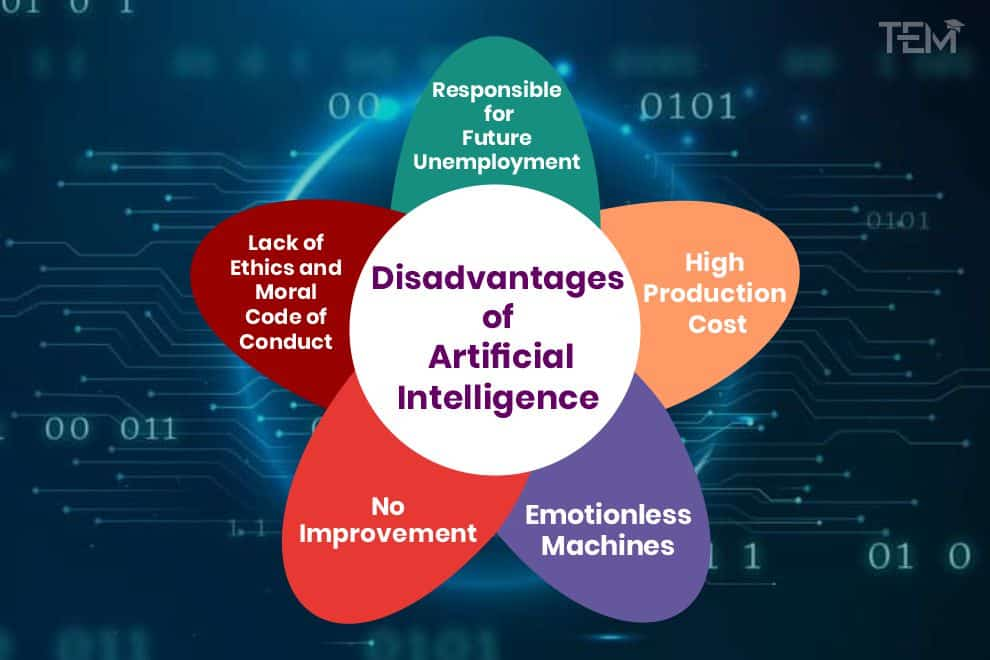
\includegraphics[width=12cm]{Disadvantages of Artificial Intelligence.jpg}\par 
 \centering
 \bf\large\caption{ Figure:Disadvantages of Artificial Intelligence}
 \noindent
 \newpage
 
\noindent
Some Examples of Famous Robots
\begin{table}[!tbh]
    \centering
        \begin{tabular}{|c|c|c}
        \hline
        \textbf{NO.} & \textbf{Famous Robots Of The World} \\
        \hline
        1 & Sophia \\
        \hline
        2 & Jia Jia \\ 
        \hline
        3 & Nadaline \\ 
        \hline
        4 & Geminoid  DK \\
        \hline
        5 & Junco Chihira \\
        \hline
        \end{tabular}
    \label{tab:1}
    \caption{\textbf{Famous Robots of the world}}
\end{table}

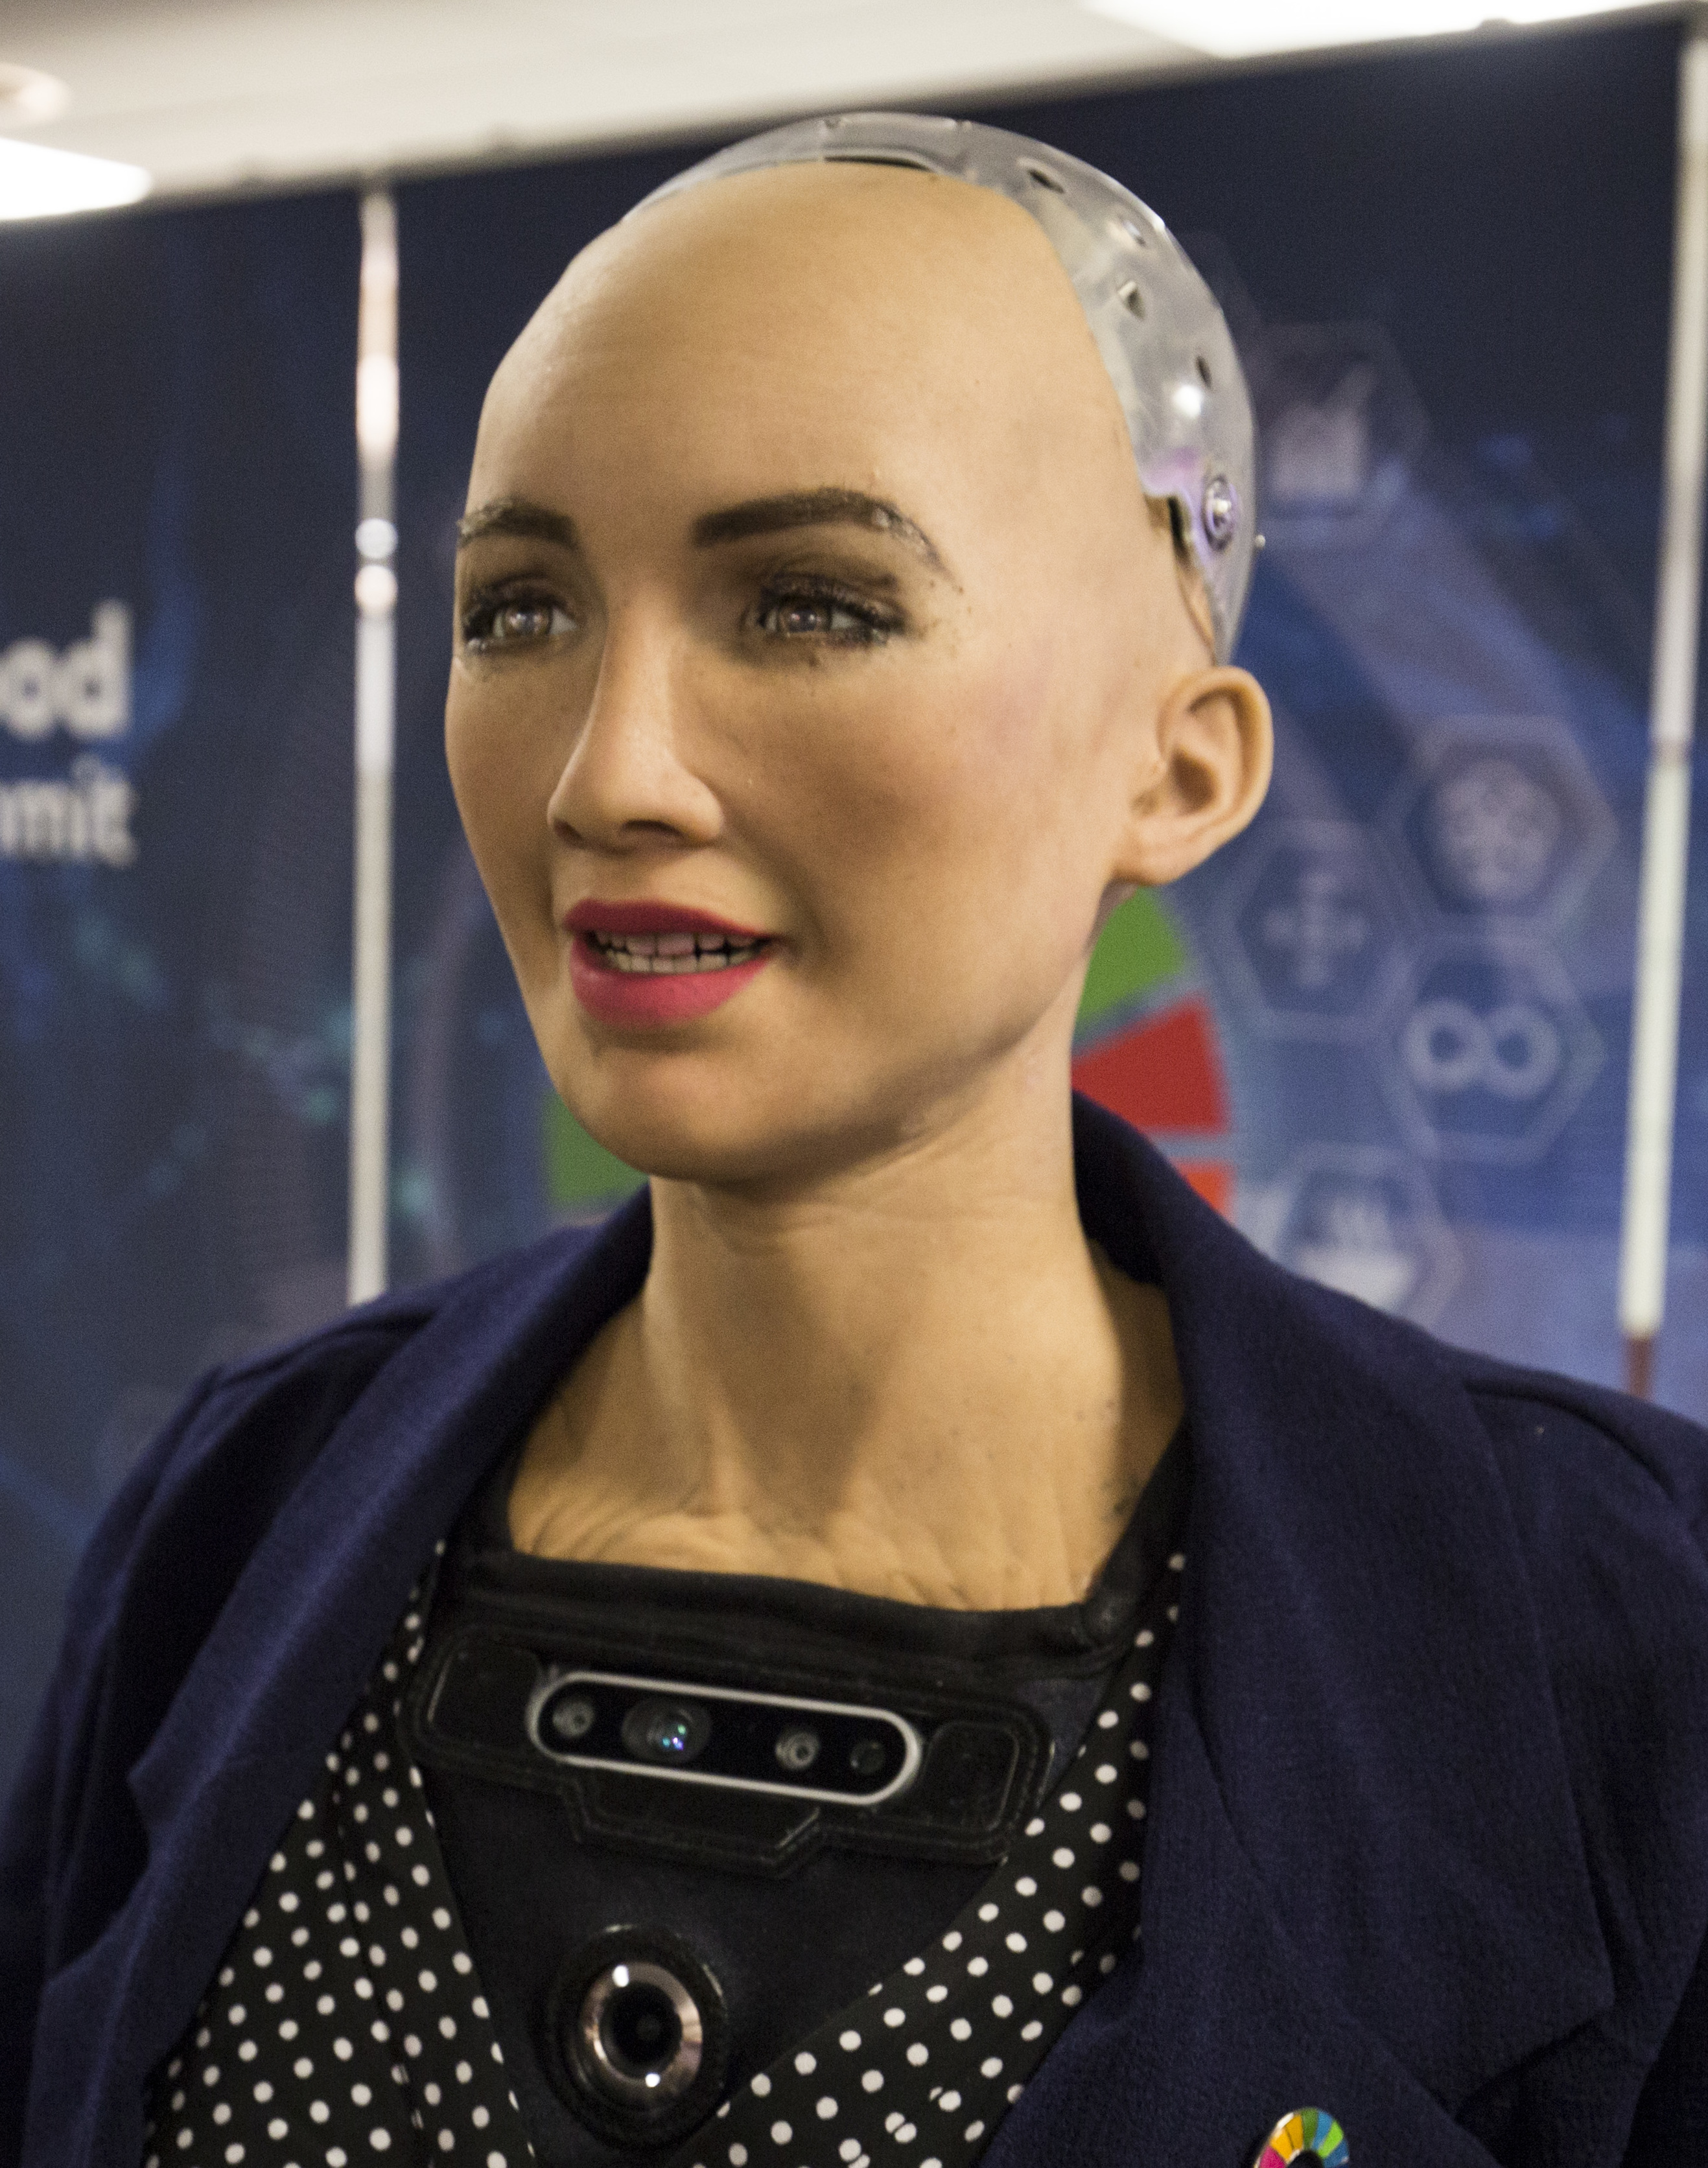
\includegraphics[width=8cm]{Sophia Robot.jpg}\par
\bf\large\caption{ Figure: Sophia robot}\par



\bf REFERENCE:-\par
1.https://www.simplilearn.com\par
2.https://en.wikipedia.org\par
3.https://www.linkedin.com\par
4.https://qbi.uq.edu.au\par


 \end{document}

 \end{document}
 



\section{Introduction}

\end{document}
